% Tactus workshop paper (expanded 4pp form).
% Target A: IROS 2026 Touch-to-Action (theme IV), deadline 2026-09-15, OpenReview, 1-4 pages.
% Target B: CoRL 2026 Small Data, Rich Sensing (short paper), deadline TBD.
\documentclass[conference]{IEEEtran}
\usepackage{graphicx}
\usepackage{booktabs}
\usepackage[hidelinks]{hyperref}

\title{Tactus: Open-Vocabulary Object Recognition\\from Low-Cost Pressure Arrays}

\author{\IEEEauthorblockN{Abdul Basit Tonmoy}
\IEEEauthorblockA{Eximius Labs\\
\texttt{atonmoy27@wabash.edu}\\
\texttt{eximiuslabs.com}}}

\begin{document}
\maketitle

\begin{abstract}
Resistive pressure arrays are the cheapest and most widely shipped tactile sensors, yet
tactile representation learning has concentrated on optical sensors that image a deforming
gel. We present Tactus, an open model that answers text queries from pressure data alone:
on the STAG benchmark (27 objects, held-out recordings), it reaches 0.771 $\pm$ 0.062 top-1
over four runs (best 0.829, top-3 0.935), matching to exceeding the 0.76 of the dataset's
supervised closed-set CNN while requiring no trained classifier head. The recipe is
deliberately small-data: 187 training recordings, masked-autoencoder pretraining on 144k
unlabeled same-sensor frames (+7 points over scratch), and the sensor's own calibration
affine, which recovered more accuracy than every architecture change combined. We report
what failed with equal precision: cross-sensor pretraining pooling produced no gain even
with per-source balancing, vision co-training degraded touch monotonically, and a
mis-normalized input pipeline silently discarded 97\% of the sensor's dynamic range while
producing plausible intermediate results. Weights, code, and the memory layer the model
plugs into are released openly.
\end{abstract}

\section{Introduction}
Touch tells a robot what vision cannot: whether a grasp holds, what is in the hand when the
camera is occluded, when contact slips. The tactile sensors most likely to ship at scale
are low-dimensional resistive and taxel arrays, which cost dollars and already appear in
gloves, insoles, and robot hands. Why, then, do tactile foundation models read only optical
sensors~\cite{fu2024tvl,higuera2024sparsh}, a signal class requiring camera-grade hardware
in every fingertip? The pressure-array side of the field has strong closed-set
classifiers~\cite{sundaram2019stag} and, recently, in-the-wild egocentric
benchmarks~\cite{song2025opentouch}, but no open model that connects the signal to
language.

Tactus fills that gap. It maps a short window of pressure frames into the frozen text
embedding space of a multimodal model (Qwen3-VL-Embedding-2B via the fusion-embedding
family~\cite{tonmoy2026fusion}), so recognition is cosine ranking against text queries.
Because the same space hosts text, image, video, audio, and inertial motion, touch becomes
one sense inside a cross-modal, language-searchable robot memory rather than an isolated
classifier.

Our contributions:
\begin{itemize}
\item An open pressure-array-to-language model that matches to exceeds STAG's supervised
closed-set baseline (0.771 $\pm$ 0.062 vs.\ 0.76 top-1) while remaining open-vocabulary
(Table~\ref{tab:results}).
\item A measured small-data recipe: sensor-calibrated normalization, cluster-sampled grasp
windows, and same-sensor masked-autoencoder pretraining, each quantified in isolation
(Table~\ref{tab:ladder}).
\item Quantified negative results, including a cross-sensor pooling ablation that
independently reproduces published cross-sensor degradation in a new sensor family
(Section~\ref{sec:negative}).
\end{itemize}

\begin{figure}[t]
\centering
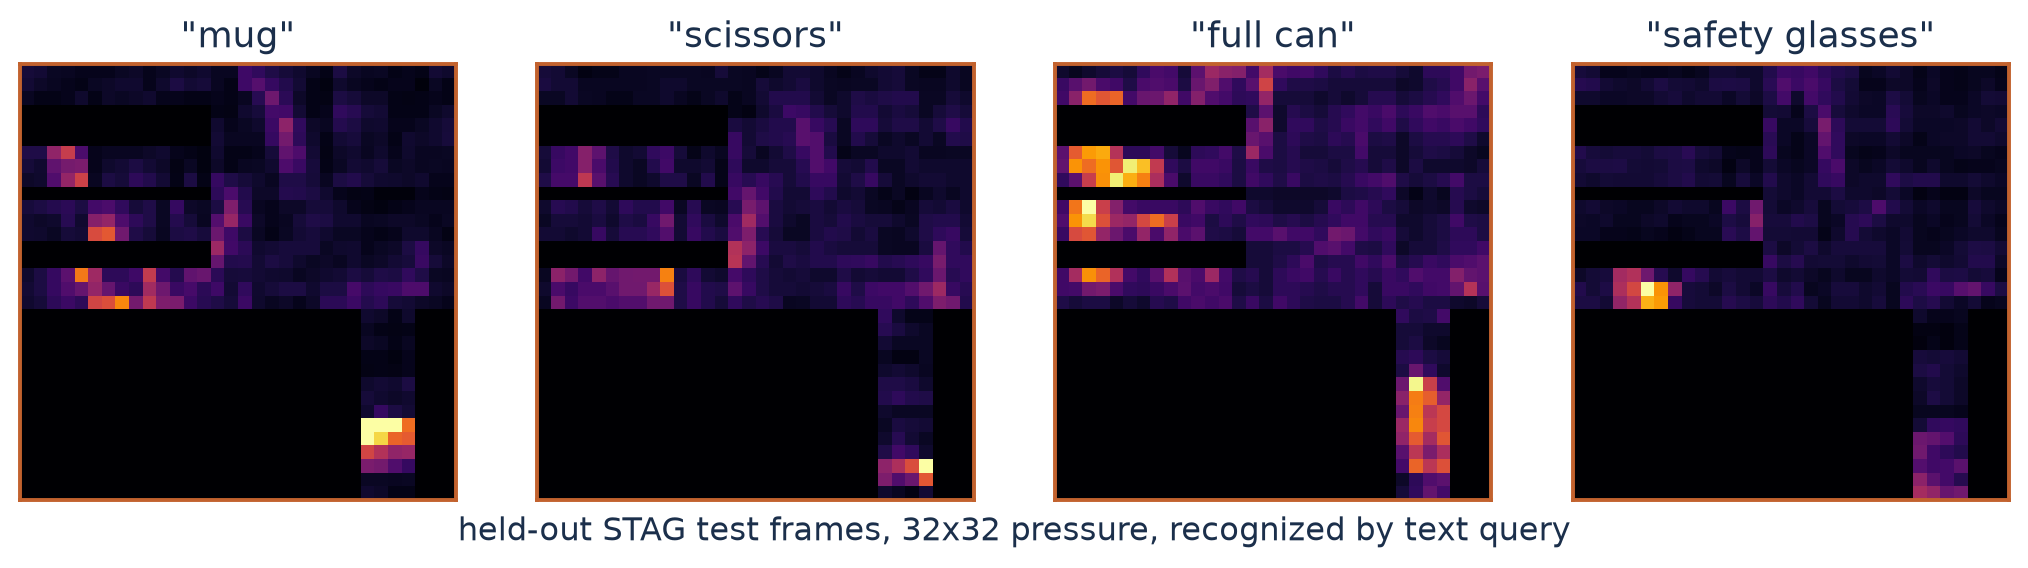
\includegraphics[width=\linewidth]{fig1_strip.png}
\caption{Tactus recognizes objects from 32$\times$32 pressure maps alone, by ranking text
queries in a shared multimodal embedding space: no camera, no trained classifier head. The
four frames are real held-out STAG test grasps with their ground-truth query phrases;
each class's most active test frame (largest total pressure) is shown. Across the full
test split the model averages 0.771 top-1 and 0.935 top-3 over 27 such queries
(Table~\ref{tab:results}).}
\label{fig:strip}
\end{figure}

\section{Related Work}
\textbf{Optical tactile representation learning.} TVL~\cite{fu2024tvl} aligns DIGIT images
with vision and language; Sparsh~\cite{higuera2024sparsh} pretrains self-supervised
representations over 460k optical tactile images; UniTouch, AnyTouch, and T3 unify multiple
camera-based sensors. All consume RGB images of a deforming elastomer through vision
backbones; none accept the low-dimensional force arrays this paper targets.

\textbf{Pressure-array recognition.} STAG~\cite{sundaram2019stag} established supervised
object recognition from a 548-taxel glove; published follow-ups reproduce rather than
exceed its accuracy on the same data. OpenTouch~\cite{song2025opentouch} contributes an
egocentric pressure-glove benchmark with cross-modal retrieval. These systems are
closed-set: recognition requires a classifier trained on the deployment vocabulary. Tactus
keeps the sensor class and removes that constraint.

\textbf{Cross-sensor tactile transfer.} HTT~\cite{bi2026htt} pretrains across
heterogeneous sensors using per-sensor encoders and balanced objectives;
TacVerse~\cite{wei2026tacverse} measures severe degradation under naive cross-sensor
transfer, even between variants of one sensor. Our pooling ablation
(Section~\ref{sec:negative}) independently reproduces this finding for pressure arrays.

\section{Method}
\textbf{Architecture.} Each 32$\times$32 frame passes through a ResNet-18-width trunk
(3$\times$3 stem, four stages); the $K{=}8$ frames of a grasp window are fused by a learned
1$\times$1 convolution over their concatenated feature maps, pooled, and projected
(512$\rightarrow$1024$\rightarrow$2048) into the frozen text space
(Fig.~\ref{fig:overview}). The head totals 16.2M trained parameters (13.5M trunk, 2.6M projector); the language side is
never updated.

\textbf{Data path.} Frames are normalized with the sensor's own calibration affine,
$\mathrm{clip}((\mathrm{raw}-500)/150,\,0,\,1)$, following the STAG reference
implementation. Training windows use STAG's cluster sampling (PCA + $k$-means per
recording, one diverse frame per cluster), which raises the effective training set from
7.7k near-duplicate windows to 62k tuples. The sibling STAG subsets (blindfolded, weights)
add 132 recordings of the same 27 objects, for 187 training recordings; test recordings
remain fully held out.

\textbf{Pretraining.} The trunk is initialized by masked-autoencoder
pretraining~\cite{he2022mae} on 144k same-sensor frames, including the 47k frames whose
labels are unusable for supervision, with mask ratio 0.6~\cite{bi2026htt} and per-patch
normalized targets; supervised test frames are excluded from the pool. Fine-tuning is label
cross-entropy at temperature 0.07 against canonical text embeddings of natural grasp
phrases (16k steps, AdamW, cosine schedule with warmup, spatial and temporal augmentation).

\textbf{Evaluation.} Test recordings are tiled into cluster tuples with a fixed seed; each
tuple is scored by cosine ranking against the 27 class phrases. We report tuple-level
top-1/top-3 and a recording-level score pooling up to 64 frames per test recording. Means
aggregate independent runs with identical hyperparameters.

\begin{figure}[t]
\centering
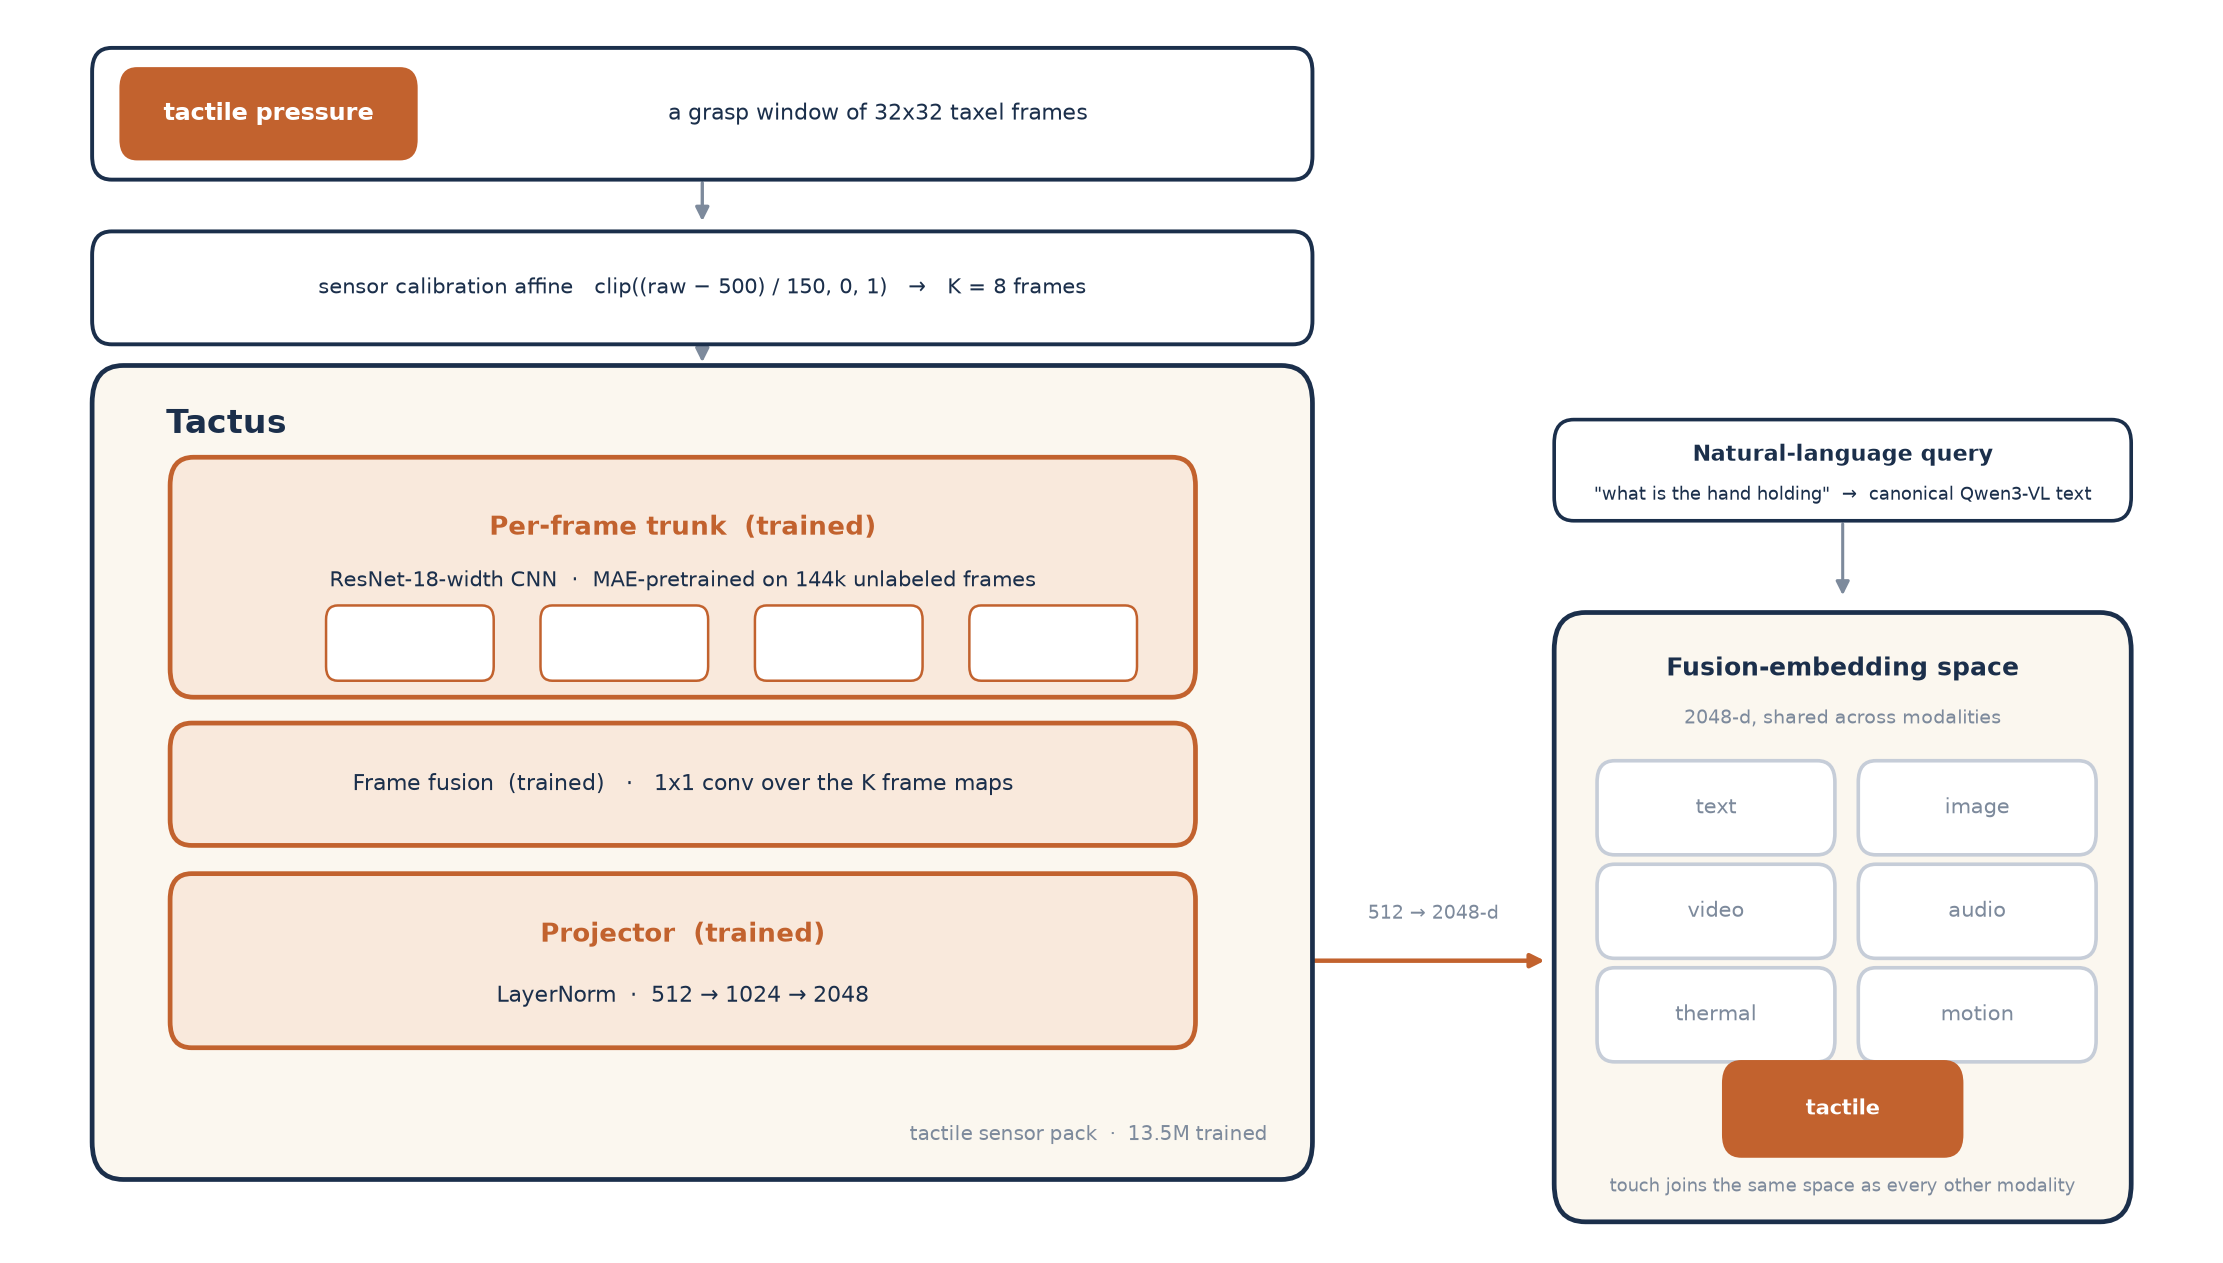
\includegraphics[width=\linewidth]{tactus_model_overview.png}
\caption{Calibrated pressure windows pass through a trained trunk, frame fusion, and
projector into a shared multimodal embedding space; recognition is a natural-language
query against the same space that hosts text, image, video, audio, and motion.}
\label{fig:overview}
\end{figure}

\section{Results}
Table~\ref{tab:results} reports 27-way recognition on STAG's held-out test recordings,
scored open-vocabulary. The recipe mean exceeds the original supervised closed-set CNN,
though by less than one standard error; we therefore characterize the result as matching to
exceeding the original baseline while performing a harder task. Top-3 accuracy is stable
across every run. Our evaluation mirrors STAG's cluster-sampling test protocol but is not
the authors' byte-identical harness.

\begin{table}[h]
\centering
\caption{STAG classification, 27 objects, held-out test recordings. Single-run rows are
marked; means carry $\pm$ one standard deviation over independent runs.}
\label{tab:results}
\begin{tabular}{lccc}
\toprule
 & top-1 & top-3 & recording top-1 \\
\midrule
Chance & 0.037 & 0.111 & 0.037 \\
STAG supervised CNN~\cite{sundaram2019stag} & 0.76 & -- & -- \\
Scratch (no MAE), mean of 3 & 0.705 $\pm$ 0.027 & 0.905 & 0.691 \\
Tactus, mean of 4 & \textbf{0.771 $\pm$ 0.062} & \textbf{0.935} & \textbf{0.722} \\
\quad best single run & 0.829 & 0.965 & 0.741 \\
\bottomrule
\end{tabular}
\end{table}

Table~\ref{tab:ladder} traces the recipe: each row is one measured change with the rest
held fixed. Data-path corrections contribute more than every architecture change combined;
the largest single step is repairing the input normalization, the second largest is
same-sensor pretraining.

\begin{table}[h]
\centering
\caption{Recipe ladder (27-way top-1). Rows above the rule predate the normalization
correction and are shown for trajectory; their absolute values are depressed by defective
input scaling.}
\label{tab:ladder}
\begin{tabular}{lc}
\toprule
Configuration & top-1 \\
\midrule
Single frames, no valid-frame filter & 0.194 \\
+ grasp windows, valid-frame filter & 0.299 \\
+ cluster sampling, conv fusion, ResNet trunk & 0.377 \\
+ cosine schedule & 0.396 \\
+ ResNet-18 width $\times$ 16k steps & 0.468 \\
+ augmentation & 0.574 \\
\midrule
Calibration affine restored (scratch, mean of 3) & 0.705 \\
+ same-sensor MAE initialization (mean of 4) & \textbf{0.771} \\
\bottomrule
\end{tabular}
\end{table}

\section{What Did Not Work}
\label{sec:negative}
Negative results shaped this recipe more than positive ones; the small-data tactile
setting makes several intuitive choices fail, and each failure below comes with the
mechanism we believe explains it.

\textbf{Cross-sensor pretraining pooling gives nothing.} Pretraining on a pool dominated
93/7 by a foreign 16$\times$16 taxel corpus produced zero downstream gain over training
from scratch, even with equal-per-source batch balancing and normalized reconstruction
targets, while same-sensor pretraining on one-thirteenth the frames was worth +7 points.
This independently reproduces, in a new sensor family, the cross-sensor degradation
reported by HTT~\cite{bi2026htt} and TacVerse~\cite{wei2026tacverse}: the trunk's features
organize around the dominant sensor's statistics, which do not transfer. Under proportional
sampling the foreign corpus additionally masked the reconstruction objective: the loss
settled at the data variance, the signature of a mean-predicting solution, which
per-patch target normalization makes visible by pinning that solution at loss 1.0.

\textbf{Vision co-training hurts touch.} Adding a contrastive touch-to-image objective
against synchronized camera frames degraded tactile recognition monotonically with its
weight (0.39 at weight 0.5, 0.28 at weight 1.0, against a 0.39 text-only control at the
time of the ablation), despite the same lever having improved our inertial-motion pack.
The mechanism we propose: the paired images are dominated by hand and scene appearance
rather than object identity, so the alignment target injects nuisance structure.

\textbf{Capacity without regularization collapses.} A from-scratch temporal-attention
encoder never left chance on 55 recordings (training loss flat at $\ln 27$); the 13.5M-trunk CNN
overfit catastrophically when trained past its optimum without augmentation; and
augmentation itself was destabilizing on a 0.9M model (three repeats spanning 0.15 to
0.48) while contributing over +10 points on the 13.5M-trunk model. Each verdict reversed with
scale, which cautions against fixed conclusions from single-configuration ablations.

\textbf{The input pipeline was the largest error source.} Our initial ingest normalized by
the corpus maximum, preserving the sensor's resting pedestal: cached frames spanned roughly
8 of 255 levels, and one sibling subset landed on a 1.5$\times$ different scale, producing
deterministic training collapses that resisted gradient clipping and temperature changes
because the optimizer was not the problem. Ablations predating this correction are reported
qualitatively above; all headline numbers postdate it. We recommend per-frame dynamic-range
checks as a standing gate for tactile pipelines: the defect was invisible in loss curves
and produced plausible intermediate accuracies for weeks of experiments.

\section{Discussion}
Three observations generalize beyond this dataset. First, in small-data tactile learning
the data path dominates: sensor calibration, frame selection, and label hygiene moved
accuracy far more than architecture. Second, self-supervision pays where labels are scarce
but frames are not: a third of our corpus was unusable for supervision yet contributed
through reconstruction pretraining. Third, transfer across tactile sensor families remains
unsolved for force arrays just as for optical sensors; treating each sensor family as its
own pretraining domain is currently the only recipe with evidence behind it. If one rule
carries over to other low-cost-sensor efforts, it is this: calibrate and diversify the
input before touching the model.

\section{Limitations and Release}
Run-to-run variance ($\pm$0.062 top-1 across four seeds, spanning 0.701 to 0.829) is the
main open engineering problem. Results cover one sensor family; our own pooling ablation
predicts that transfer to other taxel geometries requires fine-tuning. Open-vocabulary
here means text queries over the evaluation categories, not validated open-set
generalization to novel object classes. Weights (CC-BY-NC-4.0, following the training
data's license), inference code, and the Apache-2.0 session-memory layer the model plugs
into (\texttt{pip install engram-robomem}) are available via
\texttt{huggingface.co/EximiusLabs}.

\begin{thebibliography}{9}
\bibitem{sundaram2019stag}
S.~Sundaram, P.~Kellnhofer, Y.~Li, J.-Y. Zhu, A.~Torralba, and W.~Matusik,
``Learning the signatures of the human grasp using a scalable tactile glove,''
\emph{Nature}, vol. 569, pp. 698--702, 2019.

\bibitem{tonmoy2026fusion}
A.~B. Tonmoy, K.~F. Hoque, M.~S.~I. Arham, and A.~Luthra,
``Fusion embedding: A unified embedding space for text, image, video, and audio,''
\emph{arXiv:2607.18666}, 2026.

\bibitem{he2022mae}
K.~He, X.~Chen, S.~Xie, Y.~Li, P.~Doll\'ar, and R.~Girshick,
``Masked autoencoders are scalable vision learners,'' in \emph{CVPR}, 2022.

\bibitem{bi2026htt}
J.~Bi et al., ``Heterogeneous tactile transformers,'' \emph{arXiv:2606.29948}, 2026.

\bibitem{wei2026tacverse}
L.~Wei, G.~Khurana, S.~Bhouri, and D.~Zhang,
``TacVerse: A multi-sensor dataset and benchmark for cross-sensor vision-based tactile
perception,'' \emph{arXiv:2606.25877}, 2026.

\bibitem{fu2024tvl}
L.~Fu et al., ``A touch, vision, and language dataset for multimodal alignment,''
in \emph{ICML}, 2024.

\bibitem{higuera2024sparsh}
C.~Higuera et al., ``Sparsh: Self-supervised touch representations for vision-based tactile
sensing,'' in \emph{CoRL}, 2024.

\bibitem{song2025opentouch}
Y.~Song et al., ``OpenTouch: An in-the-wild egocentric tactile dataset,''
\emph{arXiv:2512.16842}, 2025.

\end{thebibliography}

\end{document}
